\subsection{Quad Merkle Tree}
A quad Merkle tree is a specific implementation of a Merkle tree used in blockchain. It is designed to be more efficient than a traditional binary Merkle tree, particularly in cases where the tree has a large number of nodes.

In a quad Merkle tree, each node has four child nodes, as opposed to two child nodes in a binary Merkle tree. This allows for faster traversal of the tree, as each level of the tree contains four times as many nodes as the previous level, rather than twice as many nodes. Additionally, a quad Merkle tree can be more efficient in terms of storage, as it requires fewer nodes to represent the same data compared to a binary Merkle tree.

\begin{figure}[H]
    \centering
    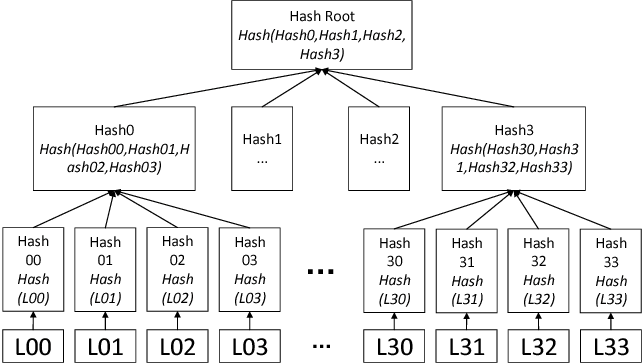
\includegraphics[scale=0.8]{figures/Quad Merkle Tree.png}
    \caption{Quad Merkle Tree}
 
\end{figure}